\doublespacing

\begin{center}
\section{Data Analysis}
\end{center}

Temperature data read from the HOBO sensors was aligned and cropped with respect to the actual trial. This prepared data included 5 sensor data sets: bottom, sample, tank and top temperatures, and flow data. Flow data was available in liters / second directly from the front panel output program. The flow data was used to locate the time frame in which the trial occured, and the temperature data was then cropped accordingly, timestamped and archived as a final trial dataset. This dataset was inserted into a spreadsheet template that performed the following analyses and calculations.

\subsection{Time Synchronization of Temperature Data}
Temperature data collected from the HOBO sensors was first synchronized in the time domain to account for vessel transience (Figure \ref{timeSync}). This amounted to a specific residency time that was primarily dependent upon the aggregate cobble size. The bottom temperature second derivative was numerically aligned with the top temperature second derivative, with the assumption that some thermal energy would be promptly measured by the bottom sensor despite thermal sinking effects. In Figure \ref{timeSync} the left plot images the first derivative of top, sample and bottom temperatures for a flow of 0.4 liters / second using a sample of glass balls (G1). The right plot is the time synchronized re-plot that results in the temperature data being temporally aligned. 

\begin{landscape}
\begin{figure}
\begin{center}
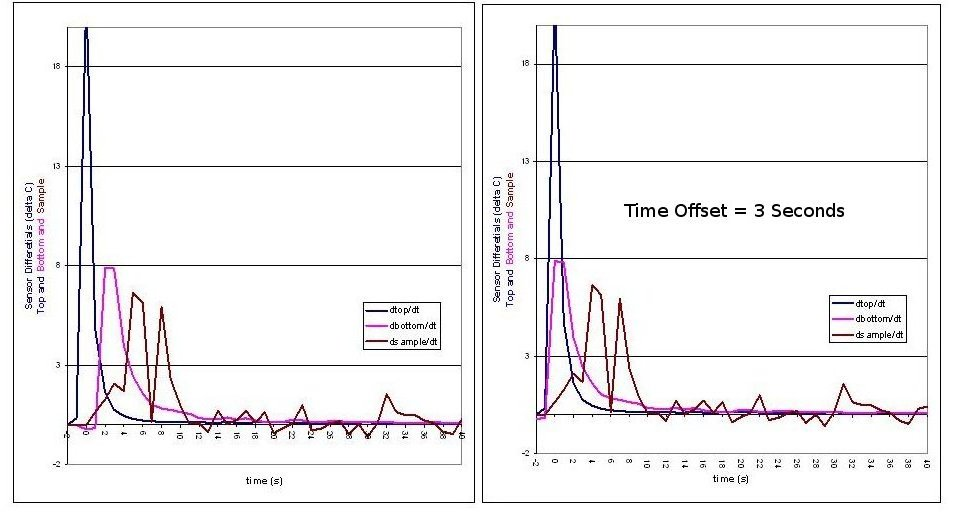
\includegraphics[scale=.6]{sideBYsideSync.jpg}
\caption[Vessel Temperature Differences]{\textbf{\emph{Non-synchronized and Synchronized Vessel Differential Temperature Data}}  The figure on the left shows first-derivative temperature data that is not time synchronized. The figure on the right shows first-derivative temperature data that has a bottom temperature shifted -3 seconds to be aligned with the top temperature readings. By aligning the rate of change of the temperature sensors, flow percolation time is removed from energy transfer anlyses.\label{timeSync}}
\end{center}
\end{figure}
\end{landscape}

\begin{landscape}
\begin{figure}
\begin{center}
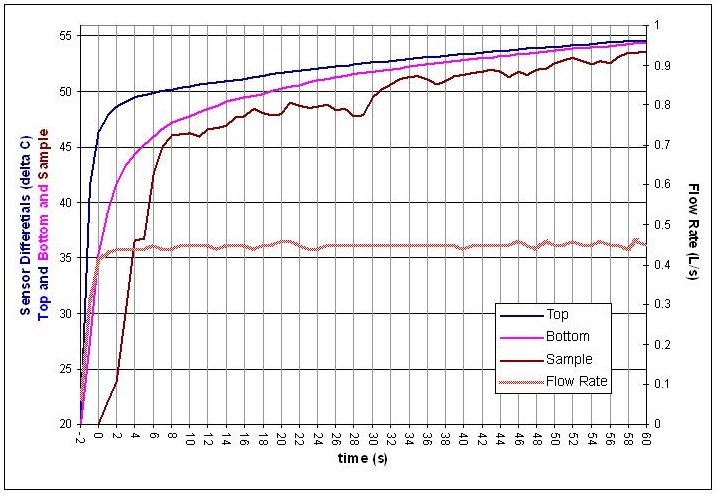
\includegraphics[scale=0.6]{timeSyncTemp.JPG}
\caption[Synchronized Temperature Data]{\textbf{\emph{Synchronized Temperature Data}}Top and Bottom temperature data is aligned in the time domain.\label{syncTemp}}
\end{center}
\end{figure}
\end{landscape}

Note that despite temporal alignment, Figure (\ref{timeSync}) illustrates a sample temperature that remains offset due to intermittent flow contact. The inflow fluid rate is insufficient to completely saturate the volume afforded by the interstitial space, and there is consequently a fractional contact between the fluid and cobbles. The noise of the sample temperature data affirms this. To intuitively align the sample data in this example, a time offset greater than the bottom offset is needed, which is physically meaningless. All temperatures and temperature differences used in analysis and theory sections has been temporally aligned with respect to vessel residency time. 

\subsection{Vessel Temperature Differential}
The synchronized temperature data was subtracted and plotted in Figure (\ref{tempDiff}).  
\[T(t)[TB]=T(t)[TOP]-T(t)[BOTTOM]\]
This quantity represents the time stepped, synchronized temperature difference across the vessel, identifying the driving potential for energy transfer. The time where this temperature difference fell below 0.12 $^{o}$C is defined as the positive thermal sink time and is denoted as $t_{+Q}$. This point identifies where the heat effectively ceases to flow from the fluid to the rock and is the key marker in performing additional analyses. The threshold of $t_{+Q}$ is determined from average sensor noise acquired during sensor calibrations and responsivity.
\pagebreak
\subsection{Cumulative Energy Transfer}
Once the data are aligned in the time domain, or synchronized, each time step is used to compute a top-bottom temperature difference. This difference is plotted over the time domain in Figure (\ref{tempDiff}). This curve is then numerically integrated according to the following theory.

\noindent The cumulative energy exchanged between the flow and the aggregate can be expressed as
\[\int \varphi T(t)dt=Q(t)[WR]\]
Where
\[\varphi = \nu_{W}Cv_{W}\]
Numerically Integrating from $t=0$ to $t_{+Q}$
\begin{equation}\label{NSCF}
\sum_{ti}^{t_{+Q}}\left[\left(\varphi\right)T(t)[TB]dt\right]=Q_{net}[WR]
\end{equation}

This method produces an integral function that can be interpreted as the cumulative energy transfer of the flow, or total heat loss from the water. The curve itself describes both the rate of energy transfer and the total quantity of thermal energy cached by the sample, and it provides the basis for further analysis of the samples' thermal sink characterization.

\begin{landscape}
\begin{figure}
\begin{center}
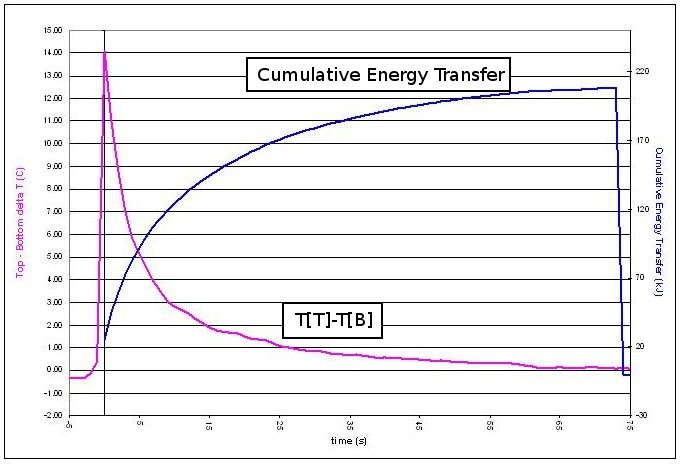
\includegraphics[scale=.65]{tempDiff.JPG}
\caption[Temperature Difference and CET Plot]{$T[T]-T[B]$ plot illustrates the temperature differences between the top and the bottom of the sample vessel along with the total thermal energy exchanged between the fluid flow and the sample - cumulative energy transfer. This example was performed with glass marbles (G1) at a flow rate of 0.40 L/s.\label{tempDiff}}
\end{center}
\end{figure}
\end{landscape}

\subsection{Normalization of the Cumulative Energy Transfer Function}
In comparisons of cumulative energy transfer (CET) functions, between different aggregates or even between different trials of the same aggregate, it is necessary to scale the data for the variances in reservoir temperature. 

\noindent From the First Law of Thermodynamics, and neglecting systemic losses,
\[-Q(t)[W]=Q(t)[R]\]
and the definition of heat transfer at constant pressure,
\[Q=mc\Delta T\]
\begin{equation}\label{specheat}
\varphi\Delta T(t)[TB]=m_{R}c_{R}\Delta T(t)[R] 
\end{equation}
The total heat lost by the fluid flow can be expressed in a time-stepped form as
\begin{equation}\label{Qt}
Q(t)[W]=[\varphi t]\Delta T(t)[TB]
\end{equation}
or as a net quantity over the entire positive thermal sink time, $t_{+Q}$
\begin{equation}\label{Qnet}
Q_{net}[W]=\varphi t\;\sum_{t=0}^{t_{+Q}}\Delta T(t)[TB]
\end{equation}
From (\ref{Qnet}) and (\ref{specheat}) the specific heat of the aggregate is computed as
\begin{equation}\label{cr}
c_{R}\;=\;\dfrac{t_{+Q}Cv_{W}\sum\Delta T(t)[TB]}{m_{R}\left(T[TOP]-T[AMBIENT]\right)}
\end{equation}
Where $T[AMBIENT]$ is used as the minimal thermal potential available at run-time and is acquired from all four temperature sensors while they are installed in the apparatus before the trial begins.

The average rock temperature as a function of time, T(t)[R] is then inferred from the time-stepped equivalent of this expression by way of the first law of thermodynamics.
\begin{equation}\label{crt}
c_{R}\;=\;\frac{t_{+Q}Cv_{W}\Delta T(t)[TB]}{m_{R}\left(T[TOP]-T[AMBIENT]\right)}
\end{equation}
and using (\ref{specheat}) with (\ref{cr})
\begin{equation}\label{rt}
T(t)[R]\;=\;\dfrac{-\Delta T(t)[TB]}{\sum\Delta T(t)[TB]}\left(2T[TOP]-T[AMBIENT]\right)
\end{equation}

Equation (\ref{rt}) is a theoretical approximation that figures aggregate temperature with respect to time is purely a function of energy exchange and heat capacties. While this is an accurate assumption, the theory section elaborates on some of the more sophisticated underpinnings that define the aggregate's thermal gradient.

A differential equation solution formulating the rate of energy exchange between the fluid and the aggregate is used as a first order approximation model of the temperature change of the aggregate. Ultimately, this will allow the data to be scaled to match other cumulative energy transfer plots for direct graphical comparison. 
\begin{equation}
\frac{T(t)[WR]}{dt}=-\sigma T(t)[WR]
\end{equation}
Where $\sigma$ is a time constant or rate of heat loss per unit time. This equation has a solution that is realized as Newton's Law of Cooling except with a reversed heat flow. The driving mechanism of thermal potential remains the same, except heat is flowing from a reservoir to a sink. 
\begin{equation}\label{dffsoln}
T(t)[WR] = T_{o}e^{-\sigma t}
\end{equation}
Where $T_{o}=T[TOP]-T[AMBIENT]$ as an initial condition of the differential solution.
This function that is used to scale is actually an algebraically simplified ratio of the form
\begin{equation}\label{simDiffEq}
\dfrac{\Delta T(t)[TB]}{\sum\Delta T(t)[TB]}\;=\;e^{-\sigma t}
\end{equation}
Where sigma represents a time constant comprised of intrinsic and environmental parameters and is elaborated on in the theory section of this document. Numerically, the left hand side of (\ref{simDiffEq}) is used to plot and compute time stepped cumulative energy transfer values.

In scaling a cumulative energy transfer function for a particular trial, the left hand side of \ref{simDiffEq} is plotted against time (Figure \ref{corrPlot}). This curve exactly mimics the shape of the cumulative energy transfer plot; however it is dimensionless and serves as a good visual comparison with other trials. 

\begin{figure}[h!]
\begin{center}
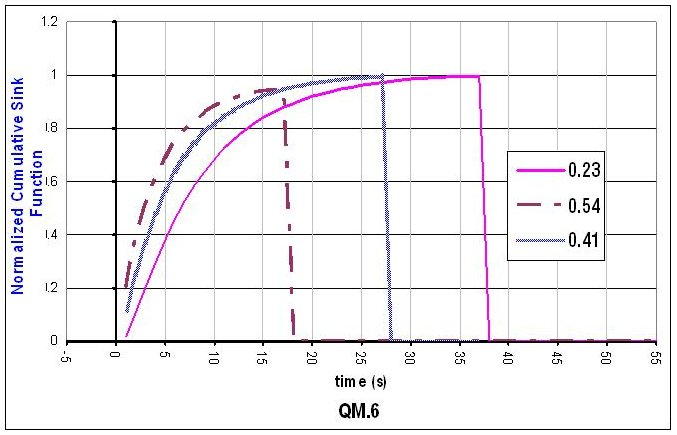
\includegraphics[scale=.6]{correctedPlot.jpg}
\caption[Normalized CET Plot]{\textbf{\emph{A Normalized Cumulative Energy Transfer Function}} An integrated or cumulative energy transfer function is shown after the scaling method summarized in Equations (\ref{rt}) and (\ref{simDiffEq}). A comparison between different sink parameters of the same aggregate can easily be interpreted from this plot.\label{corrPlot}}
\end{center}
\end{figure}

While it is tangent to the process of normalizing the cumulative energy transfer functions, it is worthwhile to point out a relationship that is derived from this formulation:
\begin{equation}\label{tt}
\frac{\Delta T(t)[WR]}{T_{o}}\;=\;\frac{\Delta T(t)[WR]}{\sum\Delta T(t)[TB]}
\end{equation}
It is important to point out a pivotal assumption in this relationship: $T(t)[WR]=T(t)[TB]$. This is of course true at $t_{+Q}$ but only true \emph{on average} over the length of the vessel between $t=0$ and $t_{+Q}$. In these calculations then, it is important to note that the aggregate as a whole is blackboxed and treated as a bulk thermal sink. In the theory section the underlying mechanics of heat exchange inside the vessel will be discussed.

\subsection{Thermal Power Calculations}
Thermal power into and out of the aggregate vessel is computed to provide a numerical conceptualization of thermal sink characteristics and intermediate calculations for other thermal parameters. The time-stepped thermal power of the water column as it flows into the vessel is computed relative to the ambient temperature.

\begin{equation}\label{pin}
P[TOP]=\left(T[TOP]-T[AMBIENT]\right)\left(\varphi (t)\right)
\end{equation}

\noindent with each time step at 1 second to dimensionally arrive at J/s.

\noindent The power out of the vessel is computed in a similar way.
\begin{equation}\label{pout}
P[BOTTOM]=\left(T[TOP]-T[BOTTOM]\right)\left(\varphi (t)\right)
\end{equation}

\noindent The thermal sink power is the difference of the power of the flow in and the power of the flow out and is on the order of several kW. 
\begin{equation}\label{tsp}
P[R]=P[TOP]-P[BOTTOM]
\end{equation}

These values are useful as thermal discharge regulations are defined in terms of net energy \citep{EPA}. In recommending aggregates for thermal sink applications, a particular cobble size and material can be selected based on similar power calculations to meet specific thermal TMDLs \citep{urban}.

\subsection{Bulk $\kappa$ and $\alpha$ Calculation}
Thermal conductivity is approximated under the assumption that heat transfer inside an individual cobble is a linear transfer rate only for a comparatively short period of time while subjected to thermal duress. This assumption is compounded by significant measurement error, and the actual thermal diffusivities are computed only as a means of comparison and experiment, and not as an actual measurement of the aggregate. It should be noted that a theoretical approach was attempted using the heat equation with a floating boundary condition to represent the bottom temperature. It was determined that such a solution was unnecessarily complex, especially when results were so effectively described by the solutions mentioned in the theory section. A heat equation solution is still possible, and may be sufficiently simplified under certain conditions to be useful in providing a reliable thermal conductivity.

For each aggregate trial, the time step that coincided with the maximum heat transfer was identified and bookended with 5 more time steps. This represented about 5 seconds of the maxium thermal transfer of the aggregate. Calculating the total energy transferred in that period of time based on heat capacities, and the characteristic radii of the cobbles, a thermal conductivity was approximated.
\begin{equation}\label{k}
\alpha=\frac{A_{c}}{A}\frac{Q[W]}{R_{s}\Delta T(t)[TB]} 
\end{equation}
Where $Q[W]$ is Equation (\ref{Qt}). The term $\dfrac{A_{c}}{A}$ is an estimated contact area, that is the fraction of available aggregate surface area that is used at any moment for thermal transfer. Experimentally, these values were calibrated using the glass and steel ball trials, as thermal conductivity for these materials is well known. However, aggregates are sure to exhibit a range of different flow characteristics because they are not ideal spheres. 

Thermal diffusivity was also calculated primarily out of experimentation and a means to establish a comparative parameter that could potentially summarize an aggregate thermal response holistically.
\begin{equation}
 \kappa=\frac{\alpha}{\rho_{bulk}c_{R}}
\end{equation}
Again, thermal diffusivities were similar to those tabulated for steel and glass on respective trials. A reliable pattern among the aggregates was also observed, but is used only for comparison in the resultant analysis.